\documentclass[crop, tikz]{standalone}

\begin{document}
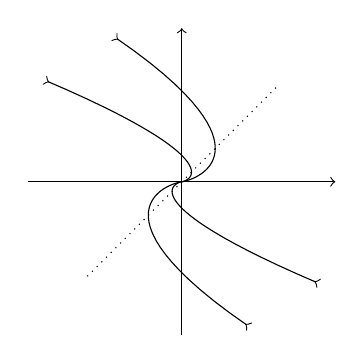
\begin{tikzpicture}[scale=1.5]
  \draw[->] (-1.3,0) -- (1.3,0);
  \draw[->] (0,-1.3) -- (0,1.3);
  \draw[>-, samples=100, domain = 0.15:10] plot ({(1.5 - \x)*exp(-\x)}, {-exp(-\x)});
  \draw[>-, samples=100, domain = 0.15:10] plot ({(-1.5 + \x)*exp(-\x)}, {exp(-\x)});
  \draw[>-, samples=100, domain = 0.2:10] plot ({(1 - 1.5*\x)*exp(-\x)}, {-1.5*exp(-\x)});
  \draw[>-, samples=100, domain = 0.2:10] plot ({(-1 + 1.5*\x)*exp(-\x)}, {1.5*exp(-\x)});
  \draw[thin, dotted] (-0.8, -0.8) -- (0.8, 0.8);
\end{tikzpicture}
\end{document}